\documentclass{article}
\usepackage{dhucs-enumerate}
\usepackage{indentfirst}
\usepackage{amsmath} % include math symbol
\usepackage{amsthm}	% include math style
\usepackage{amssymb}
\usepackage{subfig} % array the image
\usepackage{hyperref} %  hyperlink
\usepackage{xcolor} % color
\usepackage{tikz} % drawing pictures
\usepackage{multirow} % for table, make multi row
\usepackage{cancel} % cancel mark
\usepackage{mathtools} % use multlined

\textwidth 6.5 truein 
\oddsidemargin 0 truein 
\evensidemargin -0.50 truein 
\topmargin -.5 truein 
\textheight 8.5in
\setlength{\parindent}{0pt}
\hypersetup{
	colorlinks=true,
	linkcolor=red,
	filecolor=magenta,      
	urlcolor=cyan,
}


\title{Discrete Mathematics HW5}
\author{20180617 You SeungWoo}
\newcommand{\limit}[3]{\lim_{#1 \to #2} #3}
\newcommand{\firstpartial}[2]{\frac{\partial#1}{\partial#2}}
\newcommand{\highpartial}[3]{\frac{\partial^{#1}#2}{\partial#3^{#1}}}


\newenvironment{solution}
{\renewcommand\qedsymbol{$\blacksquare$}
	\begin{proof}[Solution]}
	{\end{proof}}

\theoremstyle{definition}
\newtheorem{Def}{Definition}
\newtheorem{prop}{Proposition}

\begin{document}
	\maketitle
	\section*{Problem 1}
	\begin{proof} [Solution]
		My city is Yeongju which is ranked at 72 with 108,443. The below is a population distribution of all  cities in Korea based on log scale.
		\begin{center}
			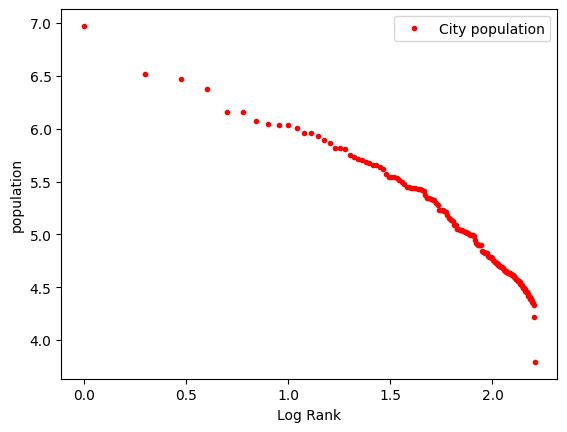
\includegraphics[width=0.5\textwidth]{pops.png}
		\end{center}
		To determine the given constants, use the linear regression to minimize the squared error.
		\begin{center}
			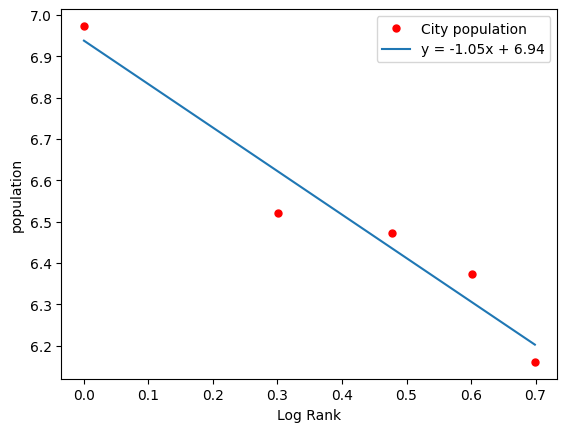
\includegraphics[width=0.5\textwidth]{pops_reg.png}
		\end{center}
		Note that I just put $C = 0$. Even though we can change $C$, it is impossible to find a value that perfectly fits the five pieces of data. By the log scale transformation, we have:
		\begin{equation*}
			\log{P(r)} = \beta \log{(r + C)} + \log{\alpha}
		\end{equation*}
		From the above line, we get
		\begin{align*}
			\beta &= -1.05\\
			\log{\alpha} &= 6.94 \Rightarrow \alpha = 10^{6.94}
		\end{align*}
		By this result, we have the relation between total cities and the line.
		\begin{center}
			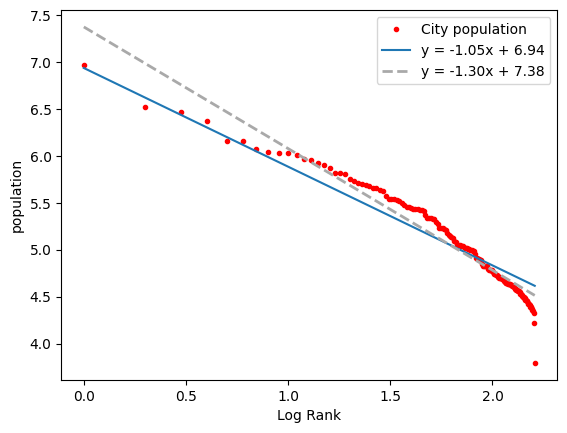
\includegraphics[width=0.5\textwidth]{pops_real.png}
		\end{center}
		The line $y = -1.30x + 7.38$ is the result of regression using all cities. They are mostly linearly distributed, but we can see that regression does not work well for some data. Clear outliers at both ends prevent Zipf\textquotesingle s law from working. Still, excluding these things, urban distribution can be explained as almost following Zipf\textquotesingle s law. There are a variety of variables that may be involved in this alignment. If there is a primate city, like Seoul, it can deviate from this rule depending on how much control it has. There may be significant differences in population depending on the level of economic and industrial growth in the region. In the case of Ulleung-gun, which is ranked last, it can be seen that the population is extremely low due to the geographical feature of being a city made up of very small islands.\\
	\end{proof}
	\section*{Problem 2}
	\begin{enumerate} [(a)]
		\item
			\begin{proof}
				Proof by induction. Consider $j = 1$. Then $H_{2} = 1 + \frac{1}{2} \geq 1 + \frac{1}{2}$ is clearly true.\\
				Suppose $j = n$ is true, consider $j = n + 1$. Then
				\begin{align*}
					H_{2^{n + 1}} &= H_{2^n} + \sum\limits_{i=1}^{2^n} \frac{1}{2^n + i}\\
					&\geq 1 + \frac{n}{2} + \sum\limits_{i=1}^{2^n} \frac{1}{2^n + i}
				\end{align*}
				If we show $\sum\limits_{i=1}^{2^n} \frac{1}{2^n + i} \geq \frac{1}{2}$, then the proof is done. Note that $\frac{1}{2^n + i} \geq \frac{1}{2^n\cdot 2}$ for $1 \leq i \leq 2^n$.
				\begin{align*}
					\sum\limits_{i=1}^{2^n} \frac{1}{2^n + i} &\geq \sum\limits_{i=1}^{2^n} \frac{1}{2^n\cdot2}\\
					&= 2^n\cdot\frac{1}{2^n\cdot 2}\\
					&= \frac{1}{2}
				\end{align*}
			\end{proof}
		\item 
			\begin{proof}
				Proof by induction. Let $P(j) = 7^{j + 2} + 8^{2j + 1}$. Consider $j = 1$. Then $7^{1 + 2} + 8^{2\cdot1 + 1} = 343 + 512 = 855 = 15\cdot57$ is clearly true.\\
				Suppose $j = n$ is true, consider $j = n + 1$. Then
				\begin{align*}
					P(n + 1) &= 7^{(n + 1) + 2} + 8^{2(n + 1) + 1}\\
					&= 7\cdot7^{n + 2} + 8^2\cdot8^{2n + 1}\\
					&= 7\cdot7^{n + 2} + 8^2\cdot8^{2n + 1} + 7\cdot8^{2n + 1} - 7\cdot8^{2n + 1}\\
					&= 7\cdot(7^{n + 2} + 8^{2n + 1}) + (8^2 - 7)\cdot8^{2n + 1}\\
					&= 7\cdot P(n) + 57\cdot8^{2n + 1}
				\end{align*}
				Since $P(n)$ is divisible by 57, the proof is done.\\
			\end{proof}
	\end{enumerate}
	
	\section*{Problem 3}
	\begin{proof}
		For any two points $a_1 = (x_1, y_1)$ and $a_2 = (x_2, y_2)$, the midpoint $z = (\frac{x_1 + x_2}{2}, \frac{y_1 + y_2}{2})$. If $\frac{x_1 + x_2}{2}$ is an integer, then $x_1$ and $x_2$ are both even or odd. Similarly, $y_1$ and $y_2$ are both even or odd. All points with integer coordinates can be classified into four sets:
		\begin{align*}
			A_1 &= \{(x, y) \mid x\mbox{ is even, } y\mbox{ is odd}\}\\
			A_2 &= \{(x, y) \mid x\mbox{ is even, } y\mbox{ is even}\}\\
			A_3 &= \{(x, y) \mid x\mbox{ is odd, } y\mbox{ is odd}\}\\
			A_4 &= \{(x, y) \mid x\mbox{ is odd, } y\mbox{ is even}\}
		\end{align*}
		If some $A_i$ has at least two elements, then we can get midpoint with integer coordinates by picking two of them. Since five distinct points are given, by the \textit{Pigeonhole Principle}, some $A_i$ has at least two elements.\\
		{\color{orange} \textbf{WARNING}}: When you classify them, using the word \textbf{group} is dangerous. Because there is a mathmatical structure called a group. Avoid using the word group unless it describes a real-life situation. We have a nice container called a set.\\
	\end{proof}
	\section*{Problem 4}
	For all problems, suppose that student choose all answers half-and-half.
	\begin{enumerate} [(a)]
		\item \begin{proof} [Solution]
			There is only one case: $_{10}\mathrm{C}_{10} = 1$(from 10 questions, select 10 correct answers). That case has $\left(\frac{1}{2}\right)^{10}\left(\frac{1}{2}\right)^0 = \left(\frac{1}{2}\right)^{10}$(10 corrects, 0 incorrects). Only about $0.098\%$.\\
		\end{proof}
		\item \begin{proof} [Solution]
			Similarly, there is only one case: $_{10}\mathrm{C}_{0} = 1$(from 10 questions, select 0 correct answers). That case has $\left(\frac{1}{2}\right)^{0}\left(\frac{1}{2}\right)^{10} = \left(\frac{1}{2}\right)^{10}$(0 corrects, 10 incorrects). Only about $0.098\%$.\\
		\end{proof}
		\item \begin{proof} [Solution]
			There are $_{10}\mathrm{C}_{1} = 10$ cases(from 10 questions, select 1 correct answer). Each case has the probability $\left(\frac{1}{2}\right)^{1}\left(\frac{1}{2}\right)^{9} = \left(\frac{1}{2}\right)^{10}$(1 correct, 9 incorrects). Therefore, the answer is $10\left(\frac{1}{2}\right)^{10}\simeq0.98\%$.\\
		\end{proof}
		\item \begin{proof} [Solution]
			There are $_{10}\mathrm{C}_{5}$ cases(from 10 questions, select 5 correct answers). Each case has the probability $\left(\frac{1}{2}\right)^{5}\left(\frac{1}{2}\right)^{5} = \left(\frac{1}{2}\right)^{10}$(5 corrects, 5 incorrects). Therefore, the answer is $_{10}\mathrm{C}_{5}\left(\frac{1}{2}\right)^{10}\simeq24.61\%$.\\
		\end{proof}
	\end{enumerate}
	\section*{Problem 5}
	\begin{enumerate} [(a)]
		\item \begin{proof} [Solution]
			There are 7 days per week. For each person, there is a $\frac{1}{7}$ chance of being born on any specific day. Also, we have $_{7}\mathrm{C}_{1} = 7$ cases to choose that specific day. Therefore, $7\times\frac{1}{7}\times\frac{1}{7} = \frac{1}{7}$\\
		\end{proof}
		\item \begin{proof} [Solution]
			First, calculate the probability that all $n$ people were born on different days of the week. The first person can be born on any of the 7 days of the week, so the probability is $\frac{7}{7}$. rom the second person onwards, they must be born on a different day than the previous person, which gives a probability of $\frac{6}{7}$. Continue this, then
			\begin{align*}
				\frac{7}{7}\times\frac{6}{7}\times\cdots\times\frac{7 - (n - 1)}{7}
			\end{align*}
			Note that this is valid for $n \leq 7$. If $n \geq 8$, then that value is 0(If you apply the \textit{Pigeonhole principle}, then the probability is 1 if $n \geq 8$). The answer is subtract it from 1.\\
		\end{proof}
		\item \begin{proof} [Solution]
			From (b), just put $n = 1$ to $7$. Here are the results.
			\begin{itemize}
				\item $n = 1\Rightarrow P = 0$ (since there's only one person, the probability of two people being born on the same day is impossible, 0)
				\item $n = 2\Rightarrow P = \frac{1}{7}$(note that this is the same as in (a))
				\item $n = 3\Rightarrow P \simeq 0.388$
				\item $n = 4\Rightarrow P\simeq 0.650$
				\item $n = 5\Rightarrow P\simeq 0.850$
				\item $n = 6\Rightarrow P\simeq 0.957$
				\item $n = 7\Rightarrow P\simeq 0.994$
				\item $n \geq 8\Rightarrow P = 1$
			\end{itemize}
			Therefore, we need at least 4 people.\\
		\end{proof}
	\end{enumerate}
	\usetikzlibrary{automata,arrows}
\section*{Problem 6}
	\begin{enumerate} [(a)]
		\item \begin{proof} [Solution]
			\mbox{}\\
			\begin{center}
				\begin{tikzpicture}
					[>=stealth', shorten >=1pt, auto, node distance=3cm, scale=1.5, transform shape]
					\node[initial, state] (A) {};
					\node[state,accepting] (C) [right of=A] {};
					\path[->] (A) edge [bend left] node [align=center] {$a$} (C)
					(C) edge [bend left] node [align=center] {$b$} (A)
					(C) edge [loop above] node [align=center] {$a$} (C)
					(A) edge [loop above] node [align=center] {$b$} (A);
				\end{tikzpicture}
			\end{center}
		\end{proof}
		\item \begin{proof} [Solution]
			\mbox{}\\
			\begin{center}
				\begin{tikzpicture}
					[>=stealth', shorten >=1pt, auto, node distance=3cm, scale=1.5, transform shape]
					\node[initial, state] (A) {};
					\node[state] (B)[above right of=A] {};
					\node[state,accepting] (C) [right of=A] {};
					\path[->] (A) edge node [align=center] {$a$} (C)
					(A) edge node [align=center] {$b$} (B)
					(C) edge [loop right] node [align=center] {$a,b$} (C)
					(B) edge [loop right] node [align=center] {$a,b$} (B);
				\end{tikzpicture}
			\end{center}
		\end{proof}
		\item \begin{proof} [Solution]
			\mbox{}\\
			\begin{center}
				\begin{tikzpicture}
					[>=stealth', shorten >=1pt, auto, node distance=3cm, scale=1.5, transform shape]
					\node[initial, state] (A) {};
					\node[state,accepting] (C) [right of=A] {};
					\path[->] (A) edge node [align=center] {$a$} (C)
					(C) edge [loop above] node [align=center] {$a,b$} (C)
					(A) edge [loop above] node [align=center] {$b$} (A);
				\end{tikzpicture}
			\end{center}
		\end{proof}
		\newpage
		\item \begin{proof} [Solution]
			\mbox{}\\
			\begin{center}
				\begin{tikzpicture}
					[>=stealth', shorten >=1pt, auto, node distance=3cm, scale=1.2, transform shape]
					\node[initial, state] (A) {};
					\node[state] (B) [above right of=A] {};
					\node[state,accepting] (C) [below right of=B] {};
					\node[state] (D) [below right of=A] {};
					\path[->] (A) edge node [align=center] {$a$} (D)
					(A) edge node [align=center] {$b$} (B)
					(B) edge node [align=center] {$a$} (C)
					(B) edge node [align=center] {$b$} (D)
					(C) edge [loop right] node [align=center] {$a,b$} (C)
					(D) edge [loop right] node [align=center] {$a,b$} (D);
				\end{tikzpicture}
			\end{center}
		\end{proof}
		\item \begin{proof} [Solution]
			\mbox{}\\
			\begin{center}
				\begin{tikzpicture}
					[>=stealth', shorten >=1pt, auto, node distance=3cm, scale=1.5, transform shape]
					\node[initial, state] (A) {};
					\node[state] (B) [right of=A] {};
					\node[state,accepting] (C) [right of=B] {};
					\path[->] (A) edge node [align=center] {$a$} (B)
					(B) edge node [align=center] {$b$} (C)
					(C) edge [loop above] node [align=center] {$a,b$} (C)
					(A) edge [loop above] node [align=center] {$b$} (A)
					(B) edge [loop above] node [align=center] {$a$} (B);
				\end{tikzpicture}
			\end{center}
		\end{proof}
	\end{enumerate}
	\section*{Problem 7}
	\begin{proof} [Solution]
		Since 5, 6, 7 are relatively prime, by the \textit{CRT}, $^{\exists!}x \in \mathbb{Z}_{5\times6\times7}$. Find 9($3\times3$) values:
		\begin{itemize}
			\item $a_i$: dividend value
			\item $M_i$: product of divisors except the self divisor $m_i$. $M_i = \frac{m_1m_2\cdots m_n}{m_i}$
			\item $y_i$: multiplicative inverse of $M_i \mod m_i$ 
		\end{itemize}
		$a_1 = 3$, $a_2 = 4$, $a_3 = 5$, $M_1 = \frac{5\cdot6\cdot7}{5} = 42$, $M_2 = \frac{5\cdot6\cdot7}{6} = 35$, $M_3 = \frac{5\cdot6\cdot7}{7} = 30$. Find any $y_i$ which satisfies $M_iy_i \equiv 1 \mod m_i$. $y_1 = 3$, $y_2 = 5$, $y_3 = 4$.\\
		Therefore, $x \equiv \sum\limits_{i = 1}^{3}a_iM_iy_i = 1678 \equiv 208 \mod 210$.\\
	\end{proof}
	\section*{Problem 8}
	\begin{proof}
		Denote that $X(G) = 1$ means the crossing number of $G$ is 1.\\
		We can find one example for $X(K_{3,3}) \leq 1$.
		\begin{center}
			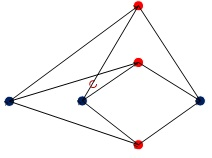
\includegraphics[width=0.4\textwidth]{K33.jpg}
		\end{center}
		If we show that $X(K_{3,3}) \neq 0$ i.e. $K_{3,3}$ is not planar, then $X(K_{3,3}) = 1$. We can prove this by applying \textit{Euler formula} as the \hyperref[problem 6]{Problem 6}. Therefore, $X(K_{3,3}) = 1$.\\
		Similarly, we can find $X(K_{3,4}) \leq 2$(note that $X(K_{4,3}) = X(K_{3,4})$).
		\begin{center}
			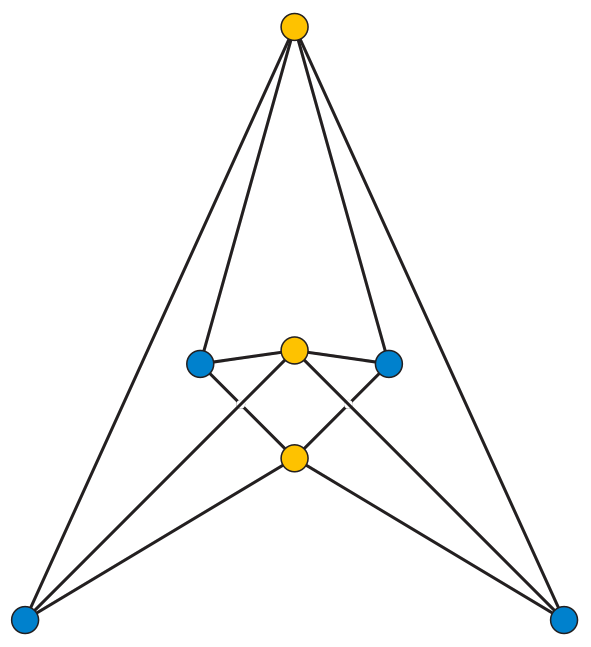
\includegraphics[width=0.4\textwidth]{K43.png}
		\end{center}
		Suppose $X(K_{3,4}) = 1$. Remove one blue vertex(in 4-node set) who occurs the crossing(note that crossing occurs between 4 vertices). Then there is no crossing, the graph forms $K_{3,3}$. i.e. $X(K_{3,3}) = 0$, contradiction. Therefore, $X(K_{3,4}) > 1$, so $X(K_{3,4}) = 2$.\\
		Similarly, we can find $X(K_{4,4}) \leq 4$.
		\begin{center}
			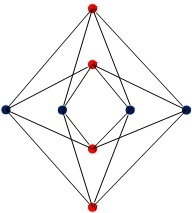
\includegraphics[width=0.4\textwidth]{K44.jpg}
		\end{center}
		Suppose $X(K_{4,4}) = 3$. Note taht crossing needs at least 4 vertices. Since $K_{4,4}$ has 8 vertices, there is at least one vertex which occurs at least 2 crossing. It is impossible to create 3 crossings with only 8 nodes so that every node participates in the crossing only once. So choose the node who occurs 2 crossing and remove it. Then the graph is $K_{3,4}$ with 1 crossing, contradiction. Therefore, $X(K_{4,4}) > 3$, so $X(K_{4,4}) = 4$.\\
	\end{proof}
	\section*{Problem 9}
	\begin{enumerate} [(a)]
		\item \begin{proof}
			Consider the below situation:
			\begin{itemize}
				\item [] Let $X$ be a set with $|X| = n$. Make a new subset of $X$ with $k$ elements, let the subset be $K$. Choose one element in $K$, let it be $\alpha$.
			\end{itemize}
			\begin{center}
				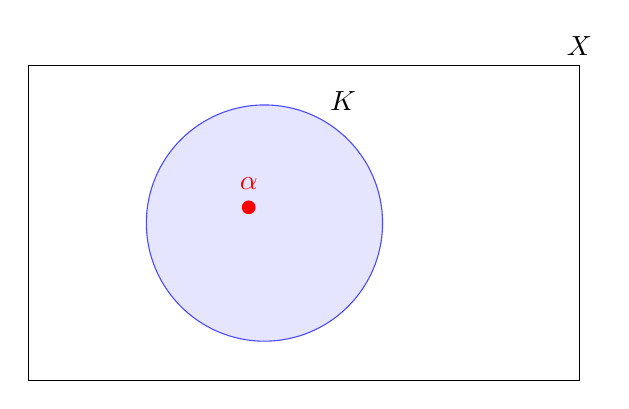
\begin{tikzpicture}
					\scope
					\clip (-4,-1) rectangle (3, 3)
					(0, 0) circle (1);
					\endscope
					\draw (-4,-1) rectangle (3, 3) node [text=black,above] {$X$};
					\draw[color=blue!70, fill=blue!10](-1, 1) circle (1.5) (0, 2.3)  node [text=black,above] {$K$};
					\draw[red, fill=red] (-1.2, 1.2) circle (0.08) (-1.2, 1.3) node [above] {$\alpha$};
				\end{tikzpicture}
			\end{center}
			There are 2 ways to make this:
			\begin{itemize}
				\item Make $K$ and choose $\alpha$ from $K$
				\item Choose $\alpha$ from $X$ and make $K$ including $\alpha$
			\end{itemize}
			The first way is $_{n}\mathrm{C}_{k}\cdot{_{k}\mathrm{C}_{1}} = k\cdot{_{n}\mathrm{C}_{k}}$ (make $K$ be $_{n}\mathrm{C}_{k}$, choose $\alpha$ be $_{k}\mathrm{C}_{1}$).\\
			The second way is $_{n}\mathrm{C}_{1}\cdot{_{n - 1}\mathrm{C}_{k - 1}} = n\cdot{_{n - 1}\mathrm{C}_{k - 1}}$ (choose $\alpha$ be $_{n}\mathrm{C}_{1}$, make $K$ be $_{n - 1}\mathrm{C}_{k - 1}$).\\
			Therefore, $k\cdot{_{n}\mathrm{C}_{k}} = n\cdot{_{n - 1}\mathrm{C}_{k - 1}}$.\\
			{\color{orange} \textbf{WARNING}}: This method is called \textit{combinatorial argument}. You {\color{red} \textbf{MUST}} tell the story in {\color{teal} \textbf{sentences}}, not in figures. Figures are not necessary, just for supporting purposes only. Drawing is not a logical explanation. If you only draw figures and do not write specific sentences, then you may get close to 0 points.\\
			{\color{cyan}\textbf{APPENDIX}}: The \textit{algebraic argument} is just calculate directly like following:
			\begin{align*}
				& k\cdot{_{n}\mathrm{C}_{k}}\\
				=\ & k\cdot\frac{n!}{k!(n - k)!}\\
				=\ & \frac{n!}{(k - 1)!(n - k)!}\\
				=\ & n\cdot\frac{(n - 1)!}{(k - 1)!(n - k)!}\\
				=\ & n\cdot\frac{(n - 1)!}{(k - 1)!(n - k)!}\\
				=\ & n\cdot\frac{(n - 1)!}{(k - 1)!(n - 1 - (k - 1))!}\\
				=\ & n\cdot{_{n - 1}\mathrm{C}_{k - 1}}
			\end{align*}
		\end{proof}
		\item \begin{proof}
			Consider the below situation:
			\begin{itemize}
				\item [] Let $X$ be a set with $|X| = n$. Make a new subset of $X$ with $r$ elements, let the subset be $R$. Make a new subset of $R$ with $k$ elements, let it be $K$.
			\end{itemize}
			\begin{center}
				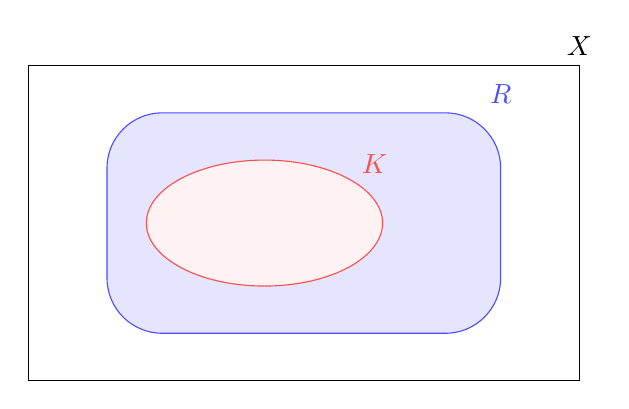
\begin{tikzpicture}
					\scope
					\clip (-4,-1) rectangle (3, 3)
					(0, 0) circle (1);
					\endscope
					\draw (-4,-1) rectangle (3, 3) node [text=black,above] {$X$};
					\draw[rounded corners=20, color=blue!70, fill=blue!10] (-3, -0.4) rectangle (2, 2.4)  node [above] {$R$};
					\draw[color=red!70, fill=red!5] (-1, 1) ellipse (1.5 and 0.8) (0.4, 1.5) node [above] {$K$};
				\end{tikzpicture}
			\end{center}
			There are 2 ways to make this:
			\begin{itemize}
				\item Make $R$ from $X$ and make $K$ from $R$
				\item Make $K$ from $X$ and make $R$ including $K$
			\end{itemize}
			The first way is $_{n}\mathrm{C}_{r}\cdot{_{r}\mathrm{C}_{k}}$ (make $R$ be $_{n}\mathrm{C}_{r}$, make $K$ be $_{r}\mathrm{C}_{k}$).\\
			The second way is $_{n}\mathrm{C}_{k}\cdot{_{n - k}\mathrm{C}_{r - k}}$ (make $K$ be $_{n}\mathrm{C}_{k}$, make $R$ be $_{n - k}\mathrm{C}_{r - k}$).\\
			Therefore, $_{n}\mathrm{C}_{r}\cdot{_{r}\mathrm{C}_{k}} = {_{n}\mathrm{C}_{k}}\cdot{_{n - k}\mathrm{C}_{r - k}}$.\\
		\end{proof}
		\item \begin{proof}
			Consider the below situation:
			\begin{itemize}
				\item [] Let $X$ be a set with $|X| = 2n$. There are 2 subsets of $X$: $A$ and $B$. They satisfy $|A| = n, |B| = n, A\cap B = \emptyset$. Make a new subset of X with $n$ elements, let the subset be $K$. Choose one element in $A\cap K$, let it be $\alpha$.
			\end{itemize}
			\begin{center}
				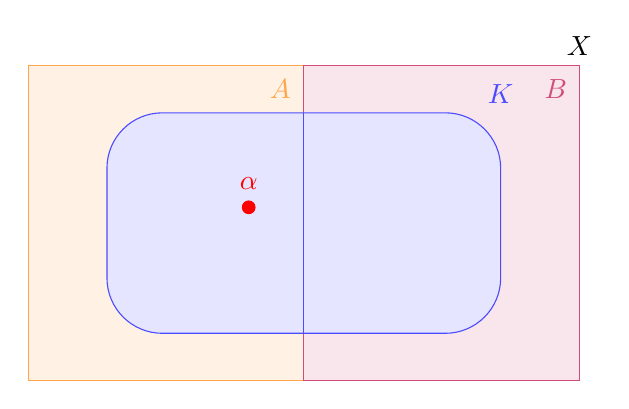
\begin{tikzpicture}
					\scope
					\clip (-4,-1) rectangle (3, 3)
					(0, 0) circle (1);
					\endscope
					\draw (-4,-1) rectangle (3, 3) node [text=black,above] {$X$};
					\draw[color=orange!70, fill=orange!10] (-4, -1) rectangle (-0.5, 3) (-0.8, 2.7) node {$A$};
					\draw[color=purple!70, fill=purple!10] (-0.5, -1) rectangle (3, 3) (2.7, 2.7) node {$B$};
					\draw[rounded corners=20, color=blue!70, fill=blue!10] (-3, -0.4) rectangle (2, 2.4)  node [above] {$K$};
					\draw[color=blue!70] (-0.5, -0.4) -- (-0.5, 2.4);
					\draw[red, fill=red] (-1.2, 1.2) circle (0.08) (-1.2, 1.3) node [above] {$\alpha$};
				\end{tikzpicture}
			\end{center}
			There are 2 ways to make this:
			\begin{itemize}
				\item Make $K$ from $X$(Choose from $A$ and $B$ each) and choose $\alpha$ from $A\cap K$
				\item Choose $\alpha$ from $A$ and make $K$ from $X$ including $\alpha$ 
			\end{itemize}
			Consider the first way. if you choose $k$ elements from $A$, then you can choose $n - k$ elements in $B$. This gives ${_{n}\mathrm{C}_{k}}\cdot{_{n}\mathrm{C}_{n - k}} = \left({_{n}\mathrm{C}_{k}}\right)^2$. This is true for $1 \leq k \leq n$. Note that $k = 0$ is impossible because we need to choose $\alpha$ in $A$. Choose $\alpha$ gives $_{k}\mathrm{C}_{1} = k$. From here, we get $\sum\limits_{k=1}^n k\left({_{n}\mathrm{C}_{k}}\right)^2$.\\
			The second way is $_{n}\mathrm{C}_{1}\cdot{_{2n - 1}\mathrm{C}_{n - 1}} = n\cdot{_{2n - 1}\mathrm{C}_{n - 1}}$ (choose $\alpha$ be $_{n}\mathrm{C}_{1}$, make $K$ be $_{2n - 1}\mathrm{C}_{n - 1}$).\\
			Therefore, $\sum\limits_{k=1}^n k\left(_{n}\mathrm{C}_{k}\right)^2 = n\cdot{_{2n - 1}\mathrm{C}_{n - 1}}$.\\
		\end{proof}
	\end{enumerate}
	\section*{Problem 10}
	\begin{proof}
		Proof by induction. Let the given statement be $P(j = r)$. Consider $P(j = 1)$. Then
		\begin{align*}
			\sum\limits_{k=0}^{1} {_{n + k}\mathrm{C}_{k}} &= {_{n}\mathrm{C}_{0}} + {_{n + 1}\mathrm{C}_{1}}\\
			&= {_{n + 1}\mathrm{C}_{0}} + {_{n + 1}\mathrm{C}_{1}}\\
			&= {_{n + 2}\mathrm{C}_{1}}
		\end{align*}
		by the \textit{Pascal\textquotesingle s rule}: $\left[{_{n}\mathrm{C}_{r}} + {_{n}\mathrm{C}_{r + 1}} = {_{n + 1}\mathrm{C}_{r + 1}}\right]$. Therefore, $P(j = 1)$ is true.\\
		Suppose $P(j = r)$ is true, consider $P(j = r + 1)$.
		\begin{align*}
			\sum\limits_{k=0}^{r + 1} {_{n + k}\mathrm{C}_{k}} &= \sum\limits_{k=0}^{r} {_{n + k}\mathrm{C}_{k}} + {_{n + r + 1}\mathrm{C}_{r + 1}}\\
			&= {_{n + r + 1}\mathrm{C}_{r}} + {_{n + r + 1}\mathrm{C}_{r + 1}}\\
			&= {_{n + r + 2}\mathrm{C}_{r + 1}}
		\end{align*}
		Therefore, $P(j = r + 1)$ is true.\\
	\end{proof}
\end{document}